\documentclass[onecolumn,11pt]{asme2ej}
\usepackage{epsfig}\usepackage{amsmath}\usepackage{amsfonts}
\usepackage{amssymb}\usepackage{graphicx}\pagenumbering{arabic}
\usepackage{verbatim}\usepackage[utf8]{inputenc}\usepackage[portuguese]{babel}
\providecommand{\keywords}[1]{\small\textbf{\textit{Keywords---}} #1}
\usepackage{comment}
\usepackage[backend=biber,style=numeric,sorting=none]{biblatex}
\usepackage{fancyhdr}\usepackage{pifont}
\usepackage{tikzsymbols}\usepackage{placeins}
\usepackage{rotating}

\pagestyle{fancy}\fancyhf{}\rfoot{Página \thepage}
\addbibresource{mybib.bib}

\title{ La'Tech Tips \\ Documento de Avaliação AHP de Projeto} 

\author{Gustavo Hammerschmidt\affiliation{PUCPR\\Ciência da Computação\\g.hammerschmidt@pucpr.edu.br}}

\author{Gustavo Foroutan Raposo \affiliation{PUCPR\\Ciência da Computação\\gustavo.raposo@pucpr.edu.br}}

\author{João Felipe Schwab Teixeira Dos Santos \affiliation{PUCPR\\Ciência da Computação\\joao.schwab@pucpr.edu.br}}

\author{Matheus Willhelm Siqueira \affiliation{PUCPR\\Ciência da Computação\\matheus.siqueira@pucpr.edu.br}}

\author{Ricardo Naoki Tanji \affiliation{PUCPR\\Ciência da Computação\\ricardo.tanji@pucpr.edu.br}}

\begin{document}

\maketitle

\FloatBarrier
\begin{figure}[h]
    \centering
    
\includegraphics[width=12cm]{LATECH/logo.PNG}
    \label{fig:spot_ini}
\end{figure}
\FloatBarrier

$\\ \\$
\FloatBarrier
\begin{table}[h]
\centering
\begin{tabular}{|l|l|l|l|}
\hline
Data       & Versão & Descrição      & Autor                 \\ \hline
05/05/2021 & 1.0    & Versão Inicial & Gustavo Hammerschmidt \\ \hline
06/05/2021 & 2.0    & Versão sem os capítulos 3, 4 e 5 & Gustavo Hammerschmidt \\ \hline
08/05/2021 & 3.0    & Versão Final & Gustavo Hammerschmidt \\ \hline
\end{tabular}
\end{table}
\FloatBarrier

\newpage
\tableofcontents
$\\ \\ $
\newpage

\section{Introdução}

Este documento retrata o processo de produção audiovisual do canal de {\it youtube} com foco em tecnologias, programação e temas voltadas à ciência da computação. La'tech Tips é um canal fictício com foco em atrair mais público à indústria tecnológica.

\section{Empresa e Problema de Decisão}

\subsection{Descrição da Empresa}

La'Tech Tips é uma empresa de produção audiovisual fictícia de um canal de {\it youtube}, focada em produzir vídeos com conteúdo sobre a área tecnológica e em atrair mais público para a indústria. Para isso, ela está interessada em dar mais foco a um dos possíveis temas de vídeo; então, usará o modelo de decisão AHP para avaliar, com base nas métricas e experiências anteriores, qual rumo dará ao canal.

\subsection{Descrição do Problema de Decisão}

A empresa se interessa por decidir qual o tema do seu próximo vídeo com base nas análises e métricas do seu canal. Para isso, ela usará o processo analítico hierárquico (AHP) para encontrá-lo.

\subsection{Critérios de Decisão}

Os critérios de decisão são as seguintes métricas:

\begin{itemize}
    \item[$*$] C1: Quantos Likes rende.
    \item[$*$] C2: Qual a estimativa porcentual de tempo de vídeo assistido.
    \item[$*$] C3: Quantas inscrições conquista.
    \item[$*$] C4: Quantos cliques na opção de receber notificações.
    \item[$*$] C5: Quantas propagandas foram vistas.
\end{itemize}

Os subcritérios de decisão são definidos abaixo para cada critério:

\begin{itemize}

    \item[$*$] SC 1.1 - Acima de 70\% das visualizações.
    \item[$*$] SC 1.2 - Entre 40 até 70\% das visualizações.
    \item[$*$] SC 1.3 - Abaixo de 40\% das visualizações.
    
    \item[$*$] SC 2.1 - Acima de 80\% das visualizações.
    \item[$*$] SC 2.2 - De 70\% até 80\% das visualizações.
    \item[$*$] SC 2.3 - Abaixo de 70\% das visualizações.
    
    \item[$*$] SC 3.1 - Acima de 10\% das visualizações.
    \item[$*$] SC 3.2 - De 2\% até 10\% das visualizações.
    \item[$*$] SC 3.3 - Abaixo de 2\% das visualizações.
    
    \item[$*$] SC 4.1 - Acima de 40\% das visualizações.
    \item[$*$] SC 4.2 - De 10\% até 40\% das visualizações.
    \item[$*$] SC 4.3 - Abaixo de 10\% das visualizações.
    
    \item[$*$] SC 5.1 - Acima de 90\% das visualizações.
    \item[$*$] SC 5.2 - De 40\% até 90\% das visualizações.
    \item[$*$] SC 5.3 - Abaixo de 40\% das visualizações.

\end{itemize}

Nas imagens obtidas das planilhas de excel, foi utilizado o nome subcritério por extenso.

\subsection{Alternativas de Decisão}

As alternativas de decisão são os seguintes temas para vídeo, cada projeto é um tema de vídeo:

\begin{itemize}
    \item[$*$] Projeto 1: Nova Linguagem de Programação.
    \item[$*$] Projeto 2: Questions \& Answers.
    \item[$*$] Projeto 3: Dicas de Linguagem.
    \item[$*$] Projeto 4: Comparação de Salários e Qualidade de Vida para Nômades.
    \item[$*$] Projeto 5: Empreendedorismo em Tech.
    \item[$*$] Projeto 6: Vlogs de Programador.
\end{itemize}

\section{Tomada de Decisão com Multicritérios}

\subsection{Considerações Gerais}

Para a construção do modelo, a equipe definiu que os pesos para os critérios e as relações das tabelas seria baseado na tabela Saaty.

\FloatBarrier
\begin{figure}[h]
    \centering
    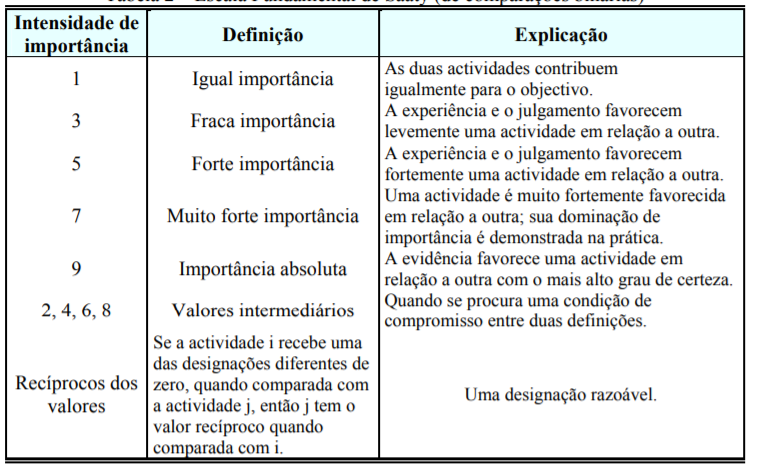
\includegraphics[width=15cm]{LATECH/tabela_saaty.PNG}
    \caption{Tabela Saaty.}
    \label{fig:sat}
\end{figure}
\FloatBarrier

\subsection{Analytic Hierarchy Process (AHP)}

O modelo AHP desenvolvido pela equipe segue a estrutura da próxima figura. Nela, cada critério está a associado a cada alternativa de projeto(tema). Para fins de visualização, devido à quantidade de flechas necessárias para indicar todas as relações, adotamos a simbologia de apenas uma relação expressando esse exato ponto.

\FloatBarrier
\begin{figure}[h]
    \centering
    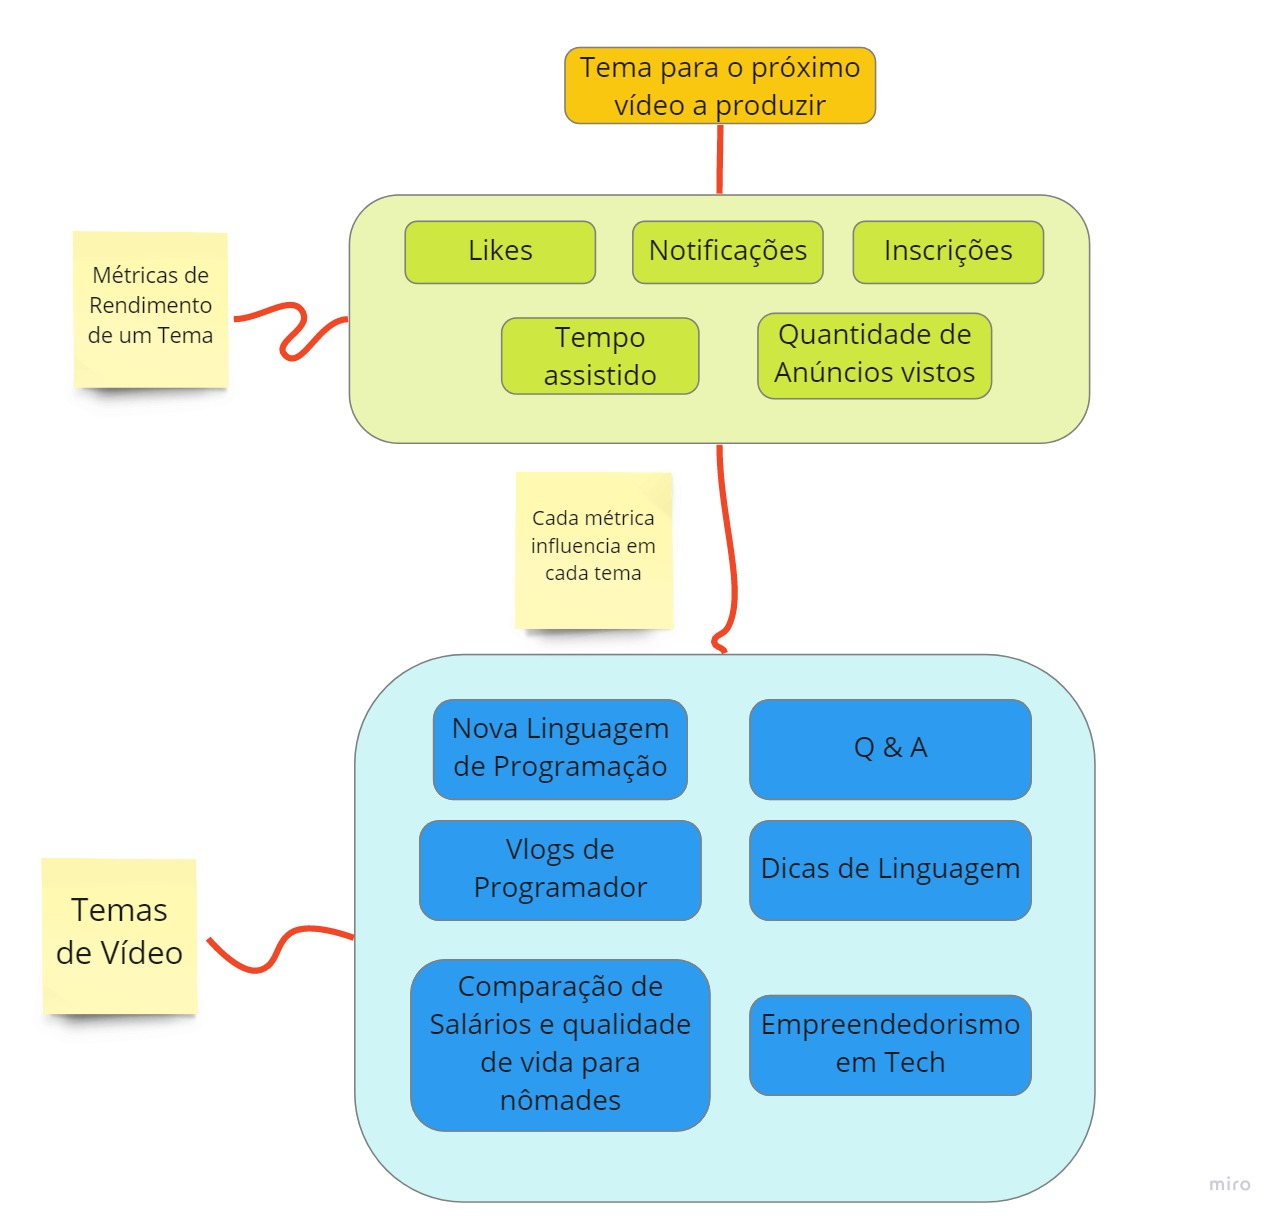
\includegraphics[width=15cm]{LATECH/AHP_model.jpg}
    \caption{Estrutura de tomada de decisão AHP.}
    \label{fig:ahp_model}
\end{figure}
\FloatBarrier

Modelo AHP com os subcritérios:

\FloatBarrier
\begin{figure}[h]
    \centering
    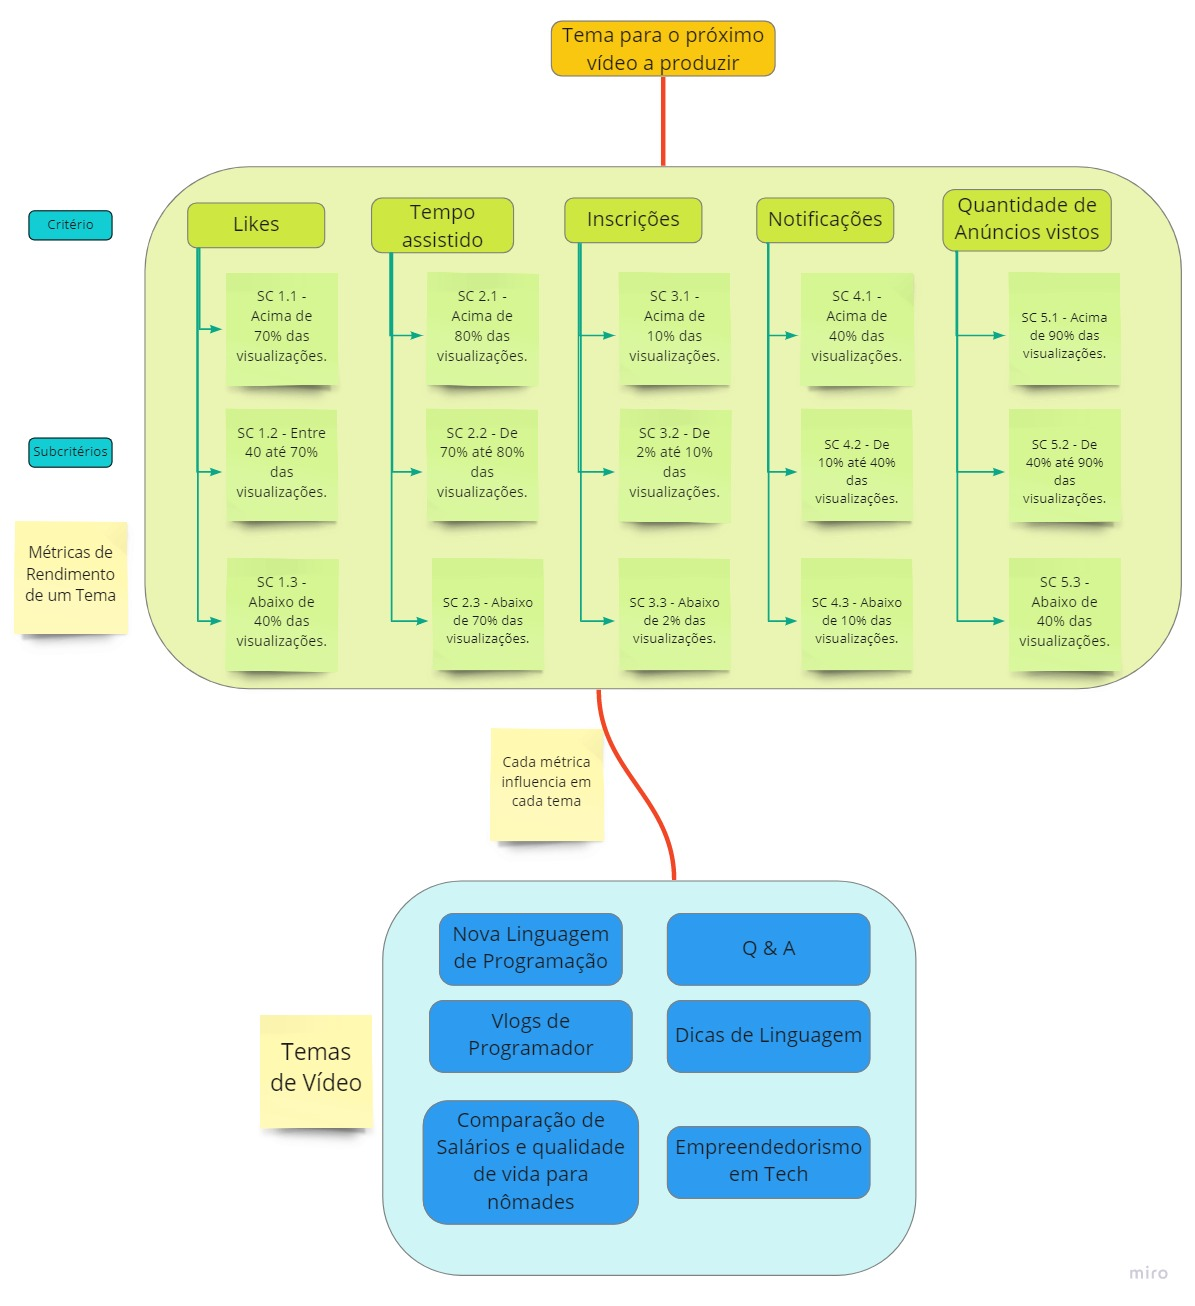
\includegraphics[width=18cm]{LATECH/modelo_adv.jpg}
    \caption{Modelo hierárquico com os subcritérios.}
    \label{fig:model_adv}
\end{figure}
\FloatBarrier

\subsection{Algoritmo para o AHP}

A execução do algoritmo da subseção anterior para a análise AHP da empresa segue os seguintes passos:


\begin{itemize}
    \item[$*$] Passo 1: Definição do peso dos critérios (C1, C2, C3, C4, C5).
    
    \item[$*$] Passo 2: Normalização das matrizes de critérios, e suas médias.
    
    \item[$*$] Passo 3: Definição dos pesos dos subcritérios e criação das matrizes; normalização da matriz, e suas médias.
    
    \item[$*$] Passo 4: Comparação dos projetos com os subcritérios.
    
    \item[$*$] Passo 5: Consolidação dos valores obtidos por subcritério para cada alternativa, soma global destes por critério e multiplicação dos critérios com a matriz de preferência por critério.
    
\end{itemize}

A geração das matrizes foi feita no excel.

\section{Modelo Multicritério de Decisão}

Utilização das métricas do canal no modelo de análise AHP.

\subsection{AHP para Hierarquização das Alternativas de Decisão}

\subsubsection{1º Nível: Critério de Decisão}

Passo 1 e Passo 2 (Definição do peso dos critérios (C1, C2, C3, C4, C5), e Normalização das matrizes de critérios, e suas médias respectivamente):

\FloatBarrier
\begin{figure}[h]
    \centering
    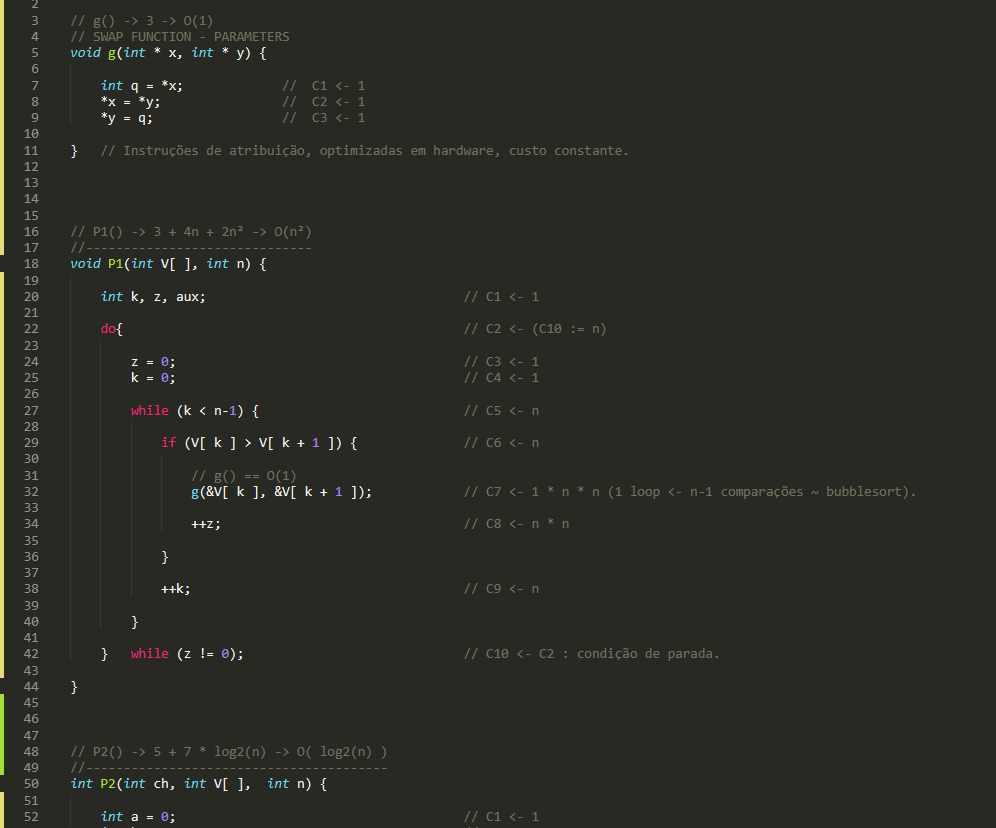
\includegraphics[width=18cm]{LATECH/p1.PNG}
     \caption{Passo 1 e Passo 2.}
    \label{fig:p_1}
\end{figure}
\FloatBarrier

\subsubsection{2º Nível: Subcritérios de Decisão de cada Critério}

Passo 3:

\FloatBarrier
\begin{figure}[h]
    \centering
    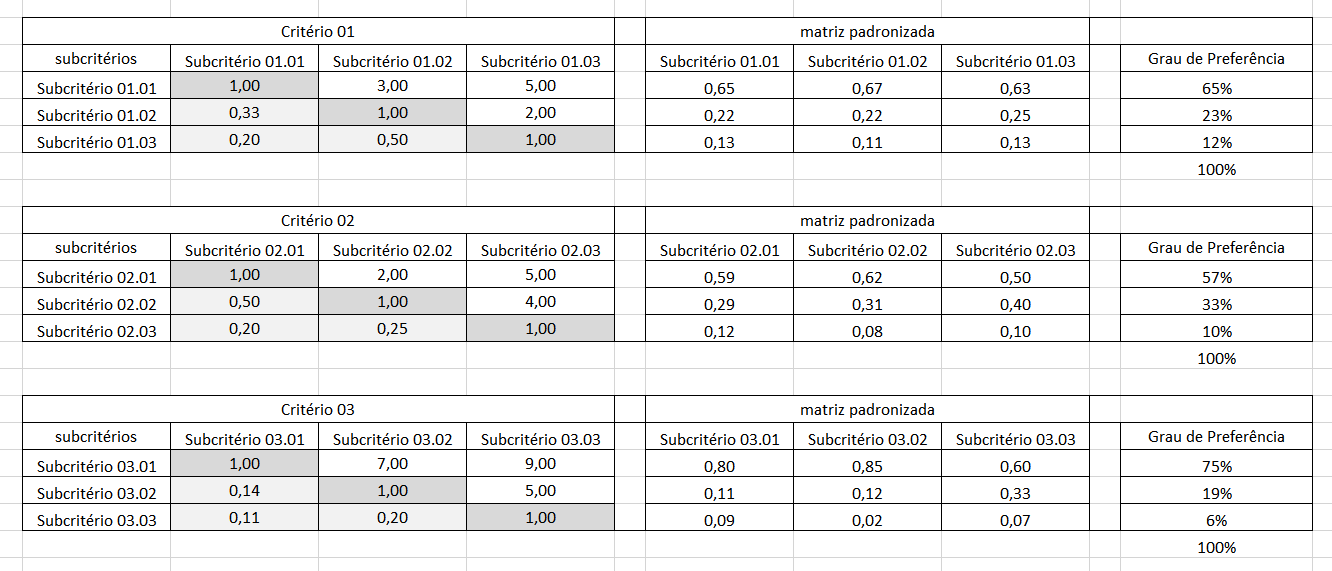
\includegraphics[width=18cm]{LATECH/p2.PNG}
     \caption{Passo 3: critérios 01, 02 e 03.}
    \label{fig:p_2}
\end{figure}
\FloatBarrier

\FloatBarrier
\begin{figure}[h]
    \centering
    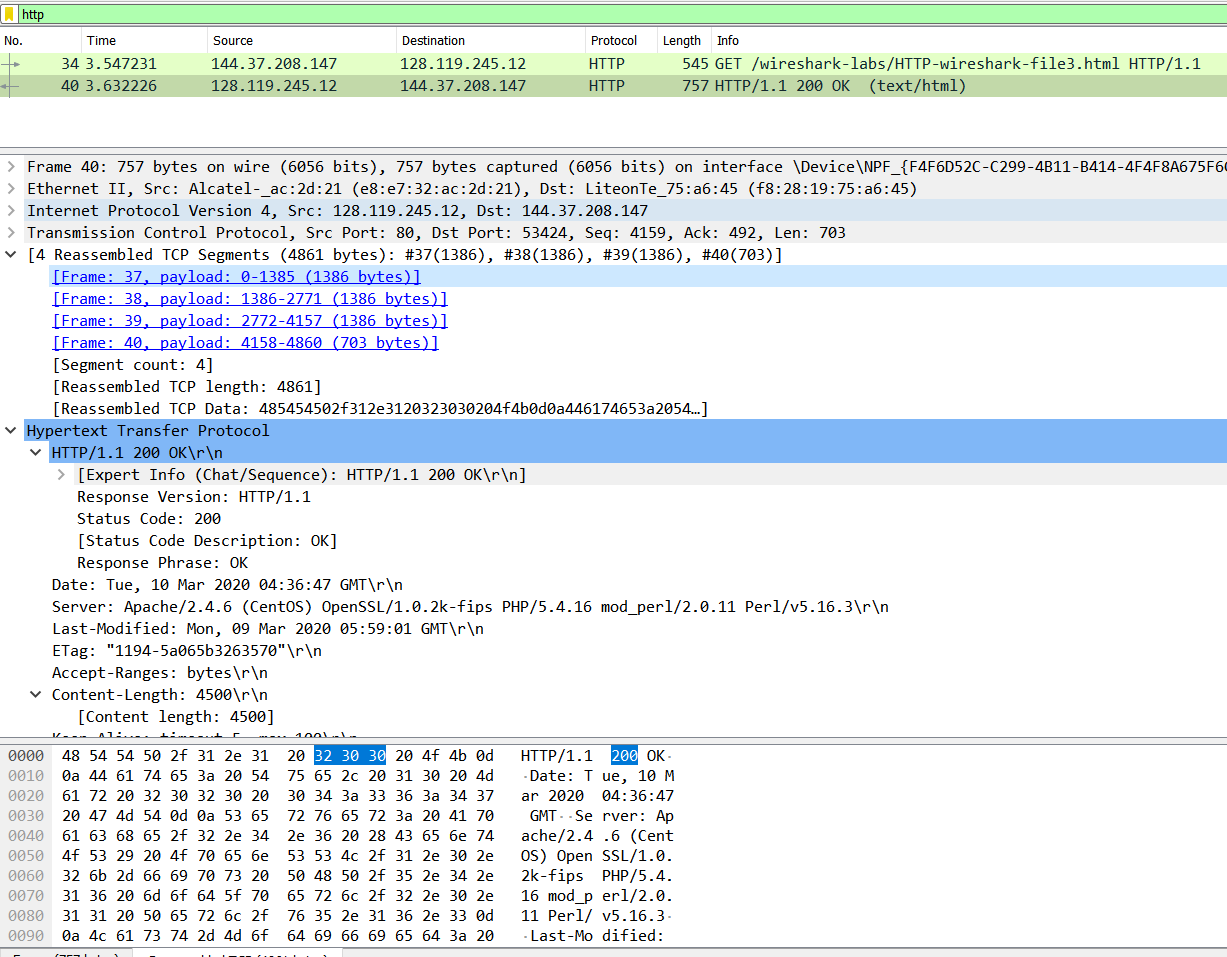
\includegraphics[width=18cm]{LATECH/p3.PNG}
    \caption{Passo 3: critérios 04 e 05.}
    \label{fig:p_3}
\end{figure}
\FloatBarrier

\subsubsection{3º Nível: Alternativas de Decisão x Subcritérios de Decisão}

Passo 4:

\FloatBarrier
\begin{figure}[h]
    \centering
    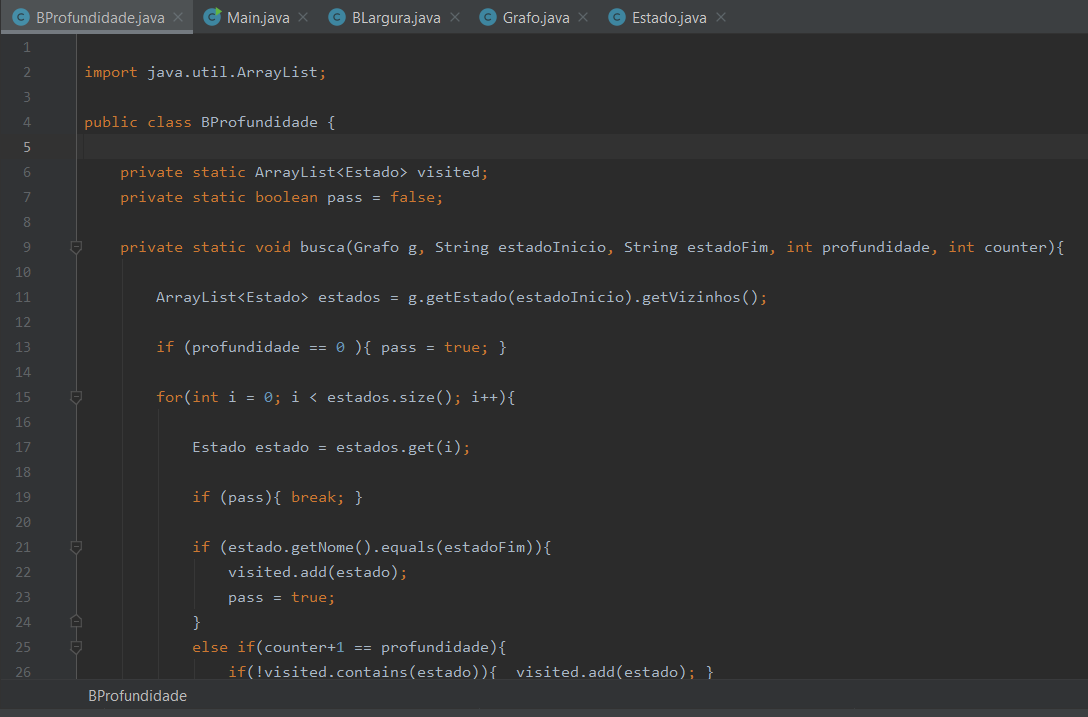
\includegraphics[width=18cm]{LATECH/b1.PNG}
    \caption{Passo 4: Critério 1.}
    \label{fig:b_1}
\end{figure}
\FloatBarrier

\FloatBarrier
\begin{figure}[h]
    \centering
    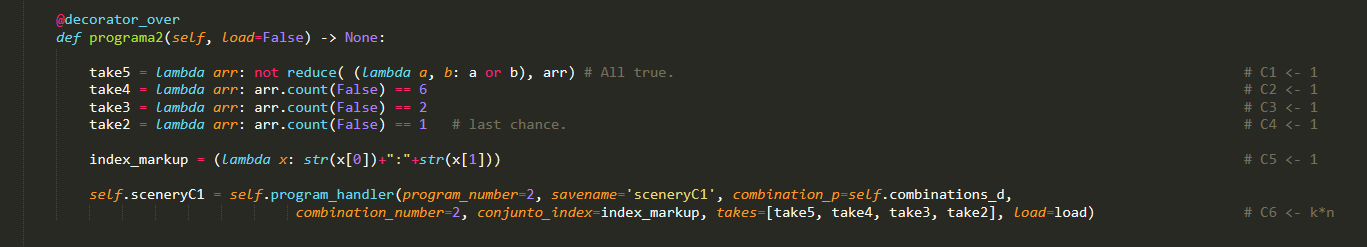
\includegraphics[width=18cm]{LATECH/b2.PNG}
    \caption{Passo 4: Critério 2.}
    \label{fig:b_2}
\end{figure}
\FloatBarrier

\FloatBarrier
\begin{figure}[h]
    \centering
    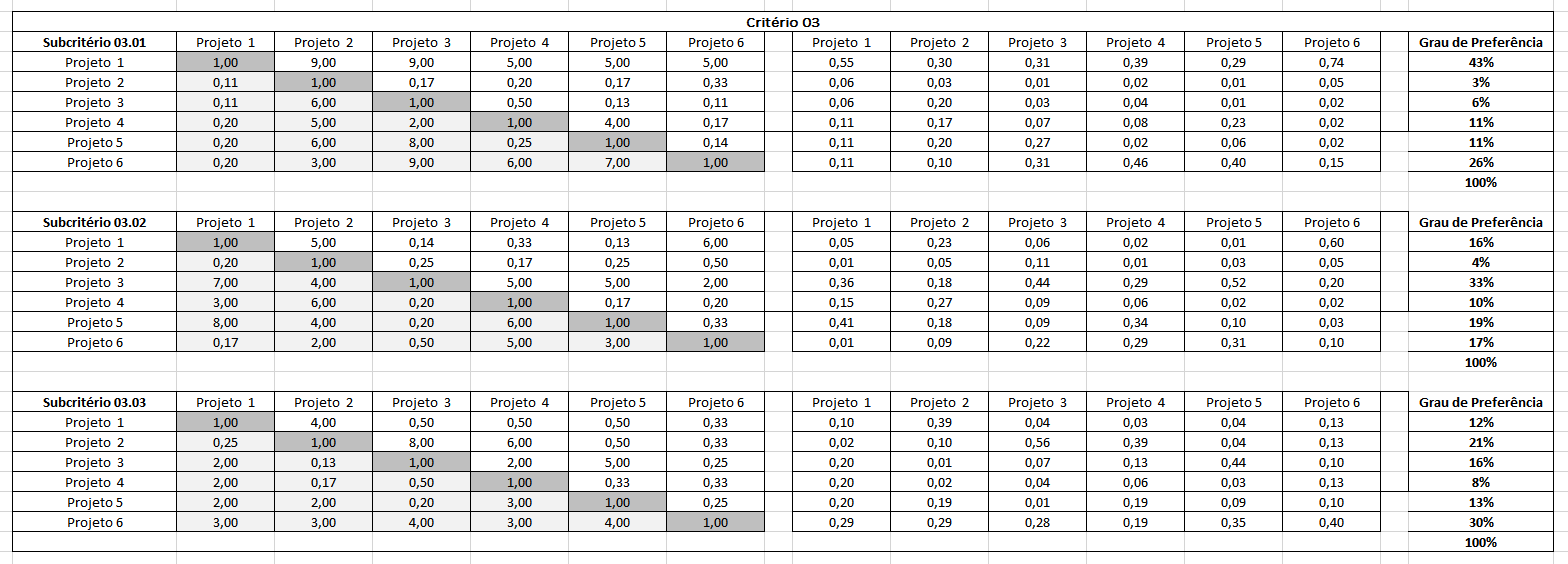
\includegraphics[width=18cm]{LATECH/b3.PNG}
    \caption{Passo 4: Critério 3.}
    \label{fig:b_3}
\end{figure}
\FloatBarrier

\FloatBarrier
\begin{figure}[h]
    \centering
    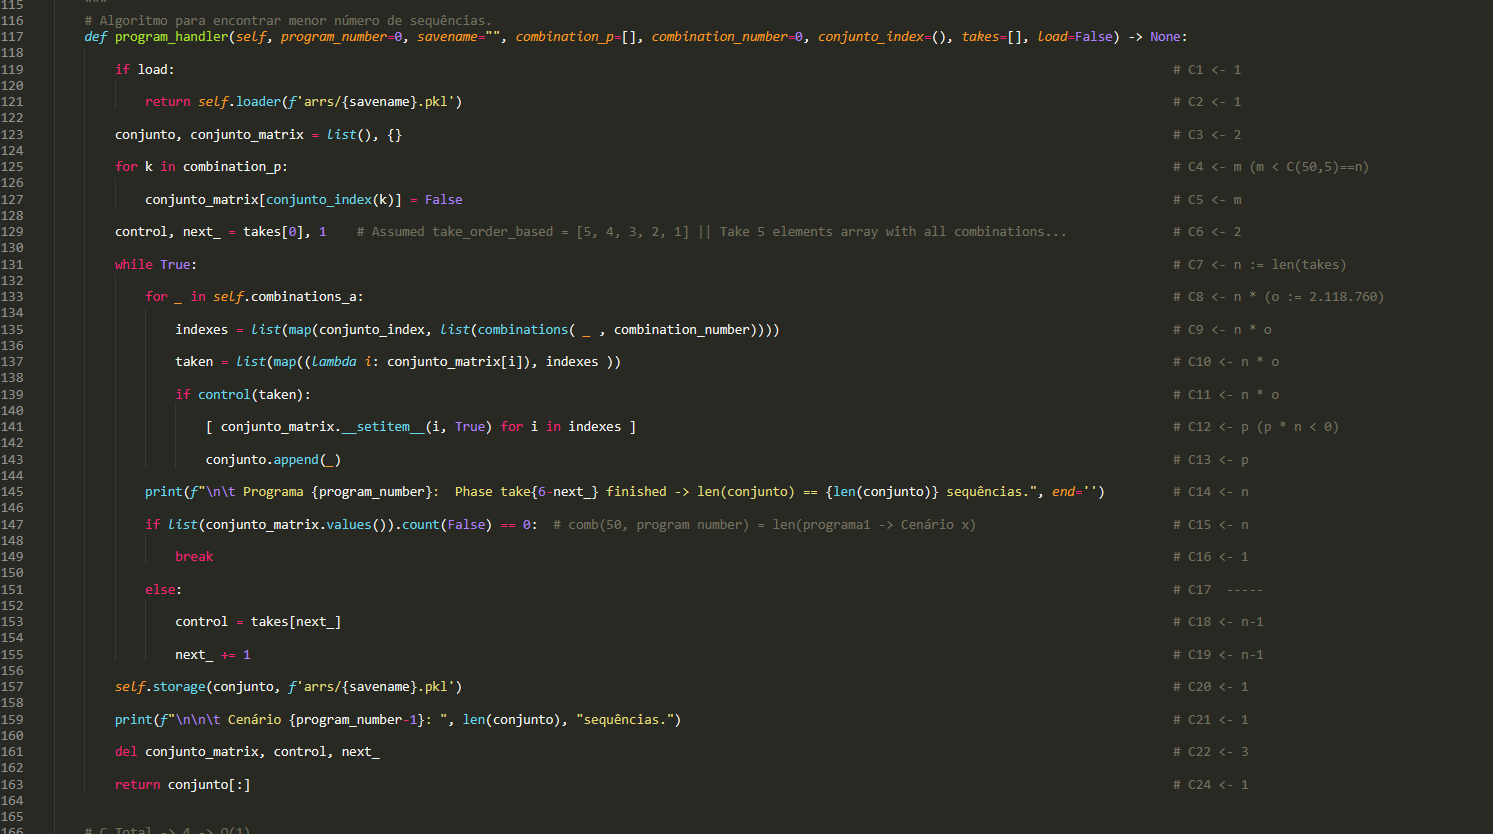
\includegraphics[width=18cm]{LATECH/b4.PNG}
    \caption{Passo 4: Critério 4.}
    \label{fig:b_4}
\end{figure}
\FloatBarrier

\FloatBarrier
\begin{figure}[h]
    \centering
    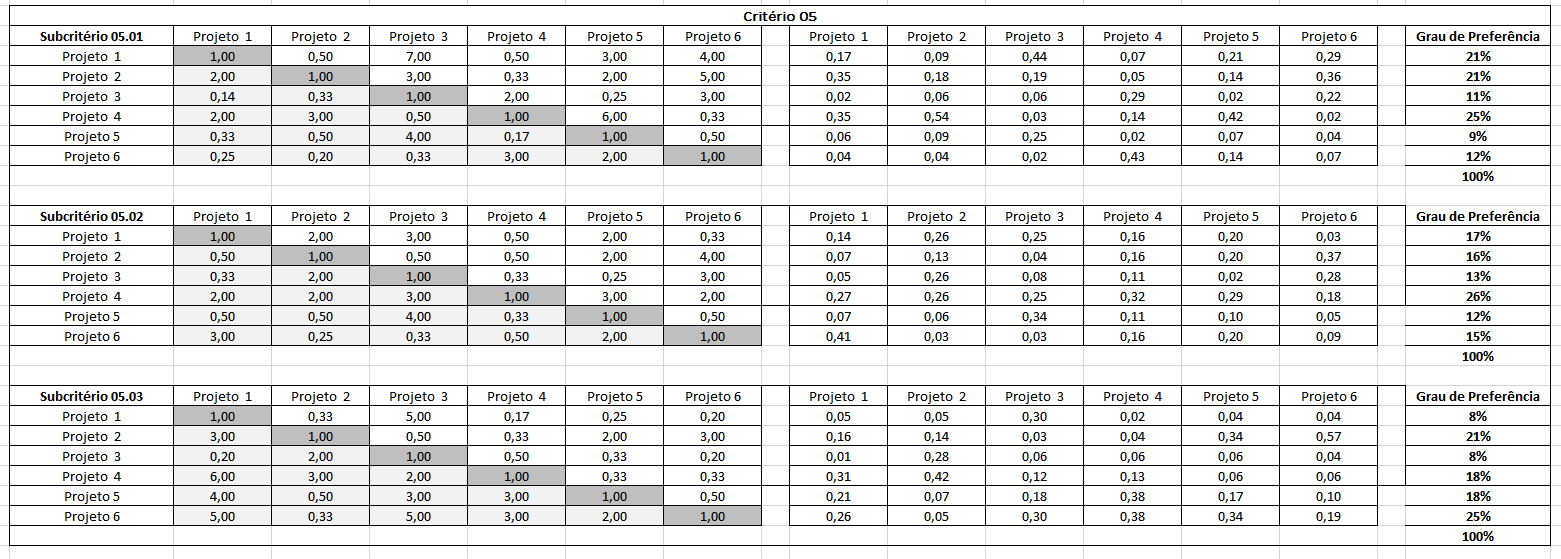
\includegraphics[width=18cm]{LATECH/b5.PNG}
    \caption{Passo 4: Critério 5.}
    \label{fig:b_5}
\end{figure}
\FloatBarrier

\subsection{Análise dos Resultados}

A análise a seguir apresenta a análise númerica obtida dos cálculos prévios -- a análise contextual se dá na conclusão. Passo 5: 

\FloatBarrier
\begin{figure}[h]
    \centering
    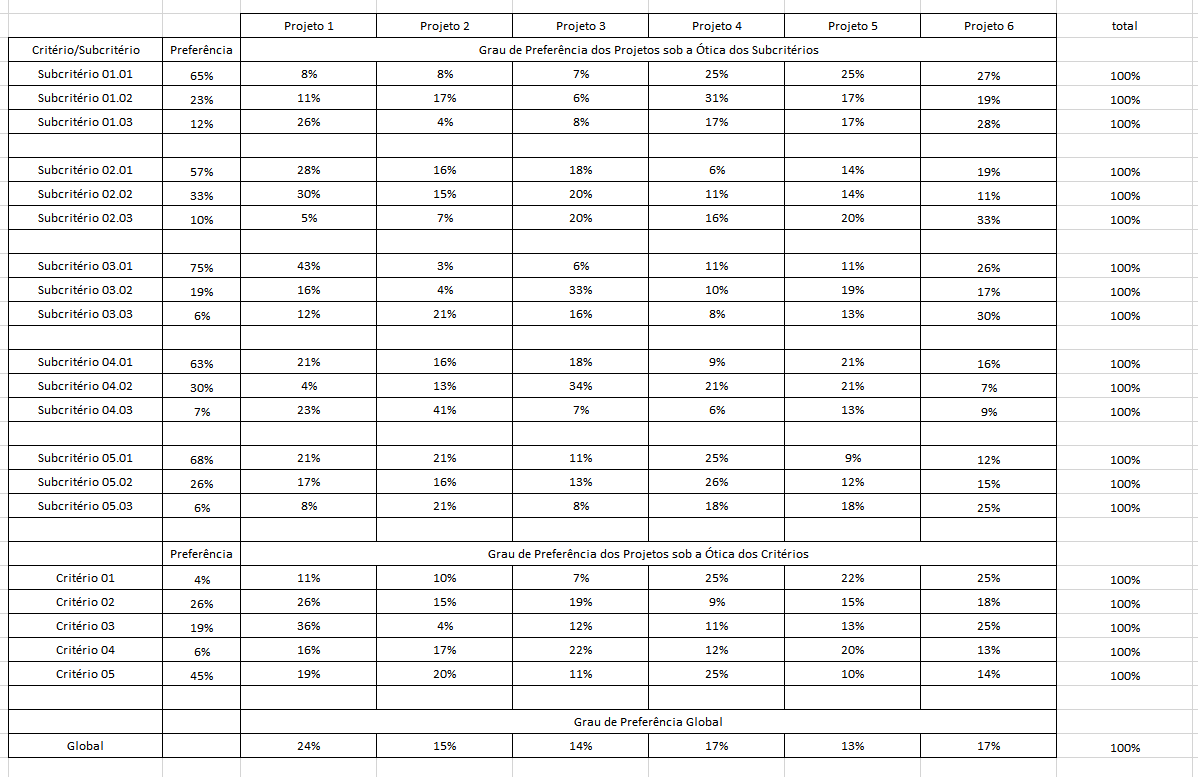
\includegraphics[width=18cm]{LATECH/anns.PNG}
    \caption{Passo 5.}
    \label{fig:ans}
\end{figure}
\FloatBarrier

\section{Conclusão}

A equipe notou que, no cenário global, o tema com maior demanda é o do projeto 1 (Nova Linguagem de programação), então, a empresa La'Tech Tips deve focar a produção de conteúdo futura na diversificação de vídeos sobre linguagens e frameworks. Também, pode ser interessante produzir vídeos com temática em comparação de salários e qualidade de vida para nômades (Projeto 4) ou vlogs e programador (Projeto 6), conteúdos que apontaram um interesse expressivo e podem ser adicionados à grade da empresa com uma menor recorrência. Nota-se que a temática empreendedorismo não é de muito gosto do público do canal na ótica global, talvez seja interessante produzir menos conteúdo e com mais qualidade pois, quanto mais likes o vídeo desta temática recebe, mais ele converte; pela a ótica de critérios, pode-se dizer o mesmo para o número de notificações: são estes dois tópicos que ajudam no bom-desempenho dessa produção (talvez, seja interessante lembrar o telespectador de clicar no sino de notificações).
Quanto ao projeto 1, o mais atrativo, deve-se manter o telespectador pelo máximo de tempo possível e pedir por sua inscrição. Para os projetos 4 e 6, os segundos mais atrativos com 17\% da preferência global, basta angariar um número significativo de likes em relação ao número de visualizações, entre 40\% a 70\% das visualizações.
Quanto aos projetos 2 e 3, 15\% e 14\% de relevância na ótica global respectivamente, pode-se utilizar dos critérios 5 e 4: aumentar o número de propagandas assistidas por vídeo e pedir para que os usuários ativem as notificações.

No entanto, ainda que possível a flexibilidade dos cursos das temáticas em novos padrões, a equipe acredita que, no curto prazo, a empresa La'Tech Tips deveria focar em aumentar sua produção dos produtos 1 (tema 1) para converter mais inscritos e monetização à sua plataforma com base nos resultados apontados pelo o modelo utilizando as métricas de desempenho do canal.

\printbibliography


\end{document}

